% filename: ProgramPlots3.tex
\documentclass[11pt]{article}
\include{PhysNote}
\usepackage{srcltx}

\usepackage{ifpdf} % to switch between .ps and .pdf file types for images (for compiling)
\usepackage{grffile} % so file.name.pdf (filename with a period in it) will be recognized as a PDF file

\title{Program Plots 3}
\author{Andrew Forrester}


\begin{document}
\maketitle
\tableofcontents


\begin{comment}
This is from ProgramPlots2.tex:

from literature, we have
  1. Tc(P)       (my fourth order fit)
  2. rho(T,P)    (my fourth order fit)
  3. alpha(T,P)  (my 6th order fit)
  4. Cp(T,P)     (my logarithmic and power fits)
  5. Cv(T,P)     (my logarithmic [and power] fits)
  6. A'(P)       (my linear fit)

vlt_K0cFind.c assumes
  1. vlt rec rel
  2. Cc value
  3. ... values...
run vlt_K0cFind.c to get
  1. Cc,K0c pairs

vlt_ThermStates.c assumes
  1. vlt rec rel
  2. ...
run vlt_ThermStates.c
  get A'(Cc)

Use A'(P) to
  get Cc(P)

vlt_K0cFind.c assumes
  1. vlt rec rel
  2. Cc value (now tied to a value of P)
  3. ... values...
run vlt_K0cFind.c to get
  1. P,Cc,K0c triples

vlt_HeatCap.c assumes
  1. vlt rec rel
  2. ...
run vlt_HeatCap.c
  get cp(T) for various P (DK0=5e-08)
      cp(T) for various P (DK0=1e-07)

vlt_ThermStates.c assumes
  1. vlt rec rel
  2. ...
run vlt_ThermStates.c
  get


\end{comment}


\section{Files}
\begin{comment}
plot_vlt_HeatCap_P_00.050_digits_13_CpVsTvDK0.ps
plot_vlt_HeatCap_P_DK0_1e-06_CpVsTv_AhlersCompare.ps
plot_vlt_HeatCap_P_DK0_1e-07_CpVsTv_AhlersCompare.ps
plot_vlt_HeatCap_P_DK0_5e-07_CpVsTv_AhlersCompare.ps
\end{comment}

\squishlist
  \item \verb|plot_vlt_HeatCap_P_DK0_1e-06_CpVsTv_AhlersCompare.ps|
  \item \verb|plot_vlt_HeatCap_P_DK0_1e-07_CpVsTv_AhlersCompare.ps|
  \item \verb|plot_vlt_HeatCap_P_DK0_5e-07_CpVsTv_AhlersCompare.ps|
\squishend



\newpage
\section{Re-runs}


\subsection{Heat Capacity}

\subsection{With different step sizes DK0}

\begin{center}
\begin{tabular}[\textwidth]{p{8cm}p{8cm}}
\ifpdf
  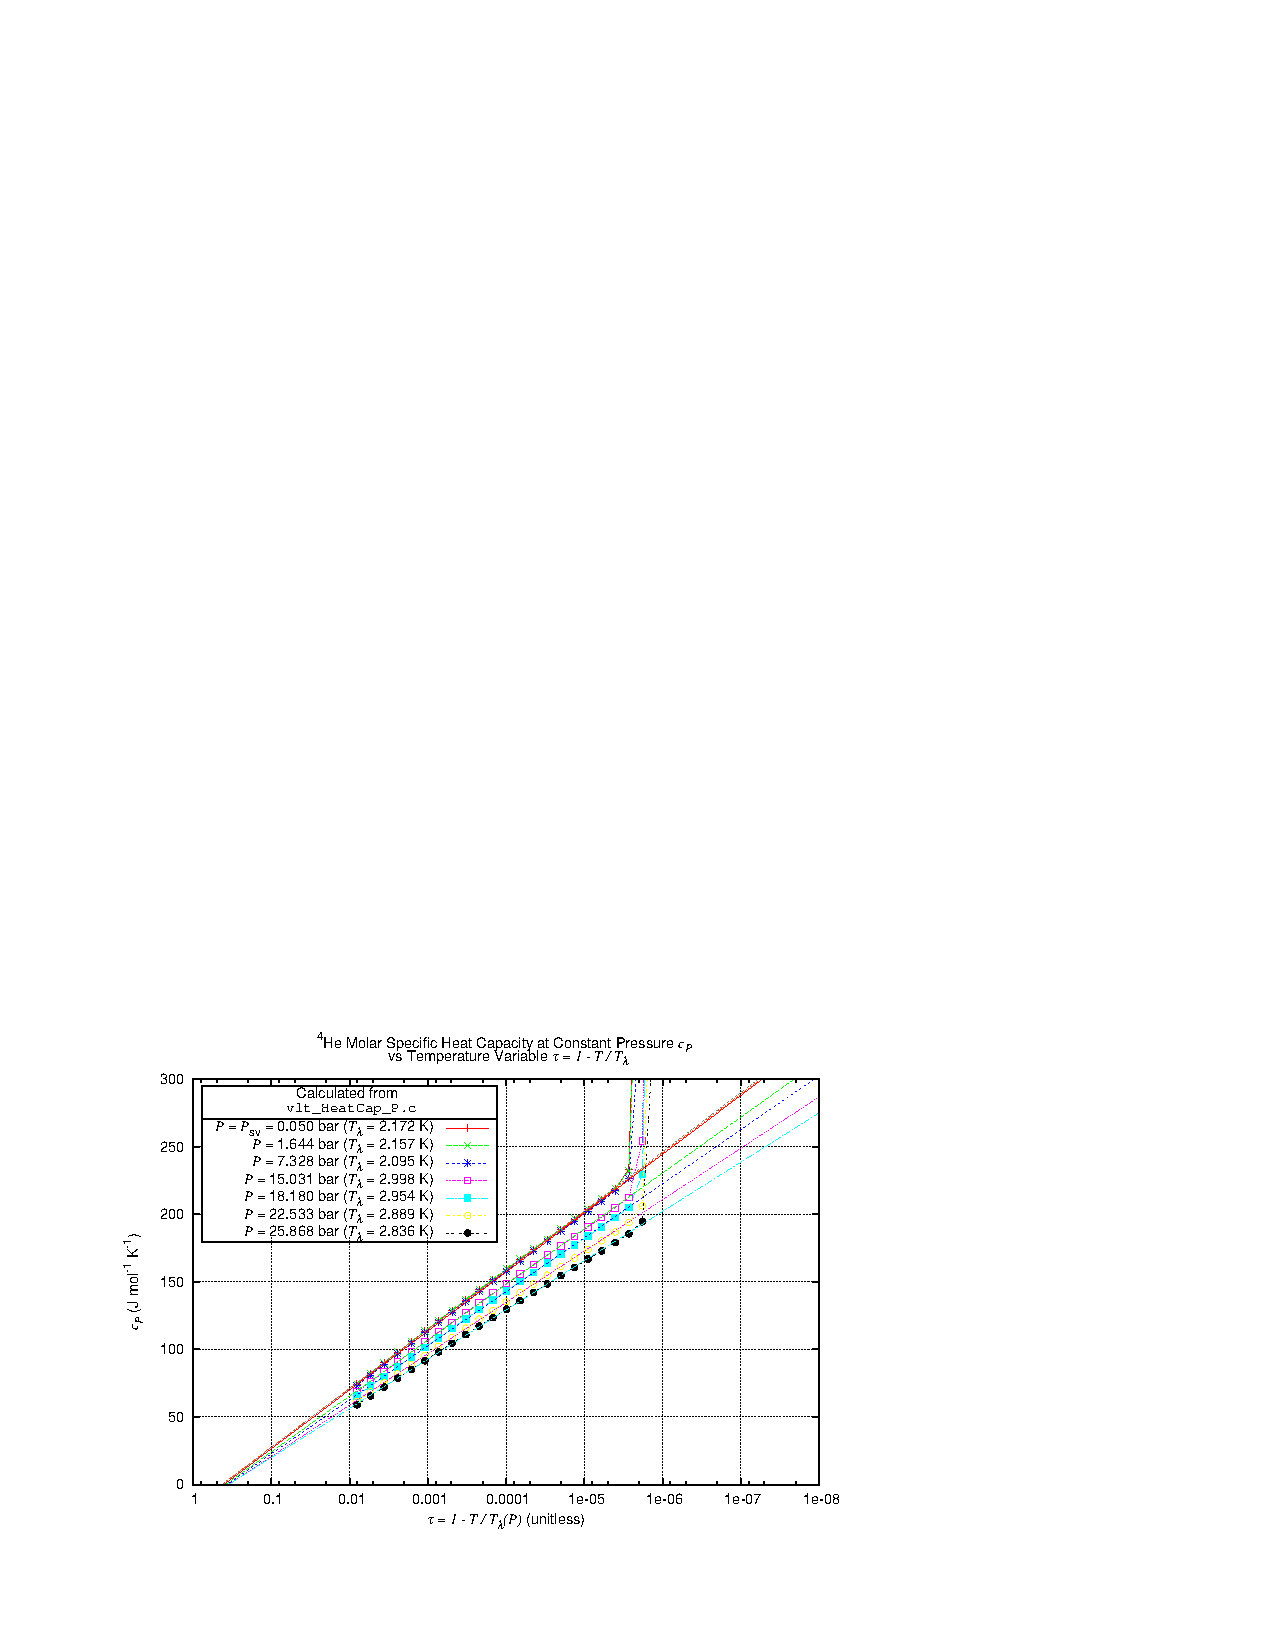
\includegraphics[width=6cm,viewport=54 53 410 300]{plot_vlt_HeatCap_P_DK0_1e-06_CpVsTv_AhlersCompare.pdf}\newline
  \verb|plot_vlt_HeatCap_P_DK0_1e-06_|\newline
  \verb|CpVsTv_AhlersCompare.pdf|
\else
  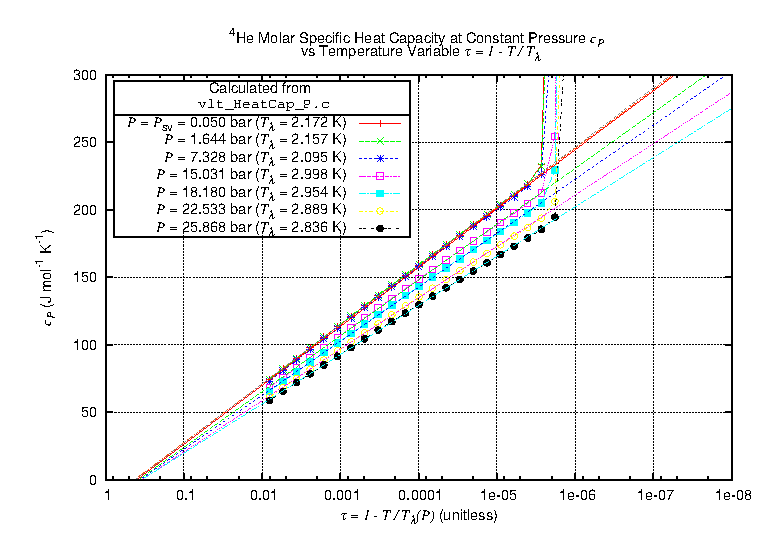
\includegraphics[width=8cm]{plot_vlt_HeatCap_P_DK0_1e-06_CpVsTv_AhlersCompare.ps}\newline
  \verb|plot_vlt_HeatCap_P_DK0_1e-06_|\newline
  \verb|CpVsTv_AhlersCompare.ps|
\fi
&
 \\
\ifpdf
  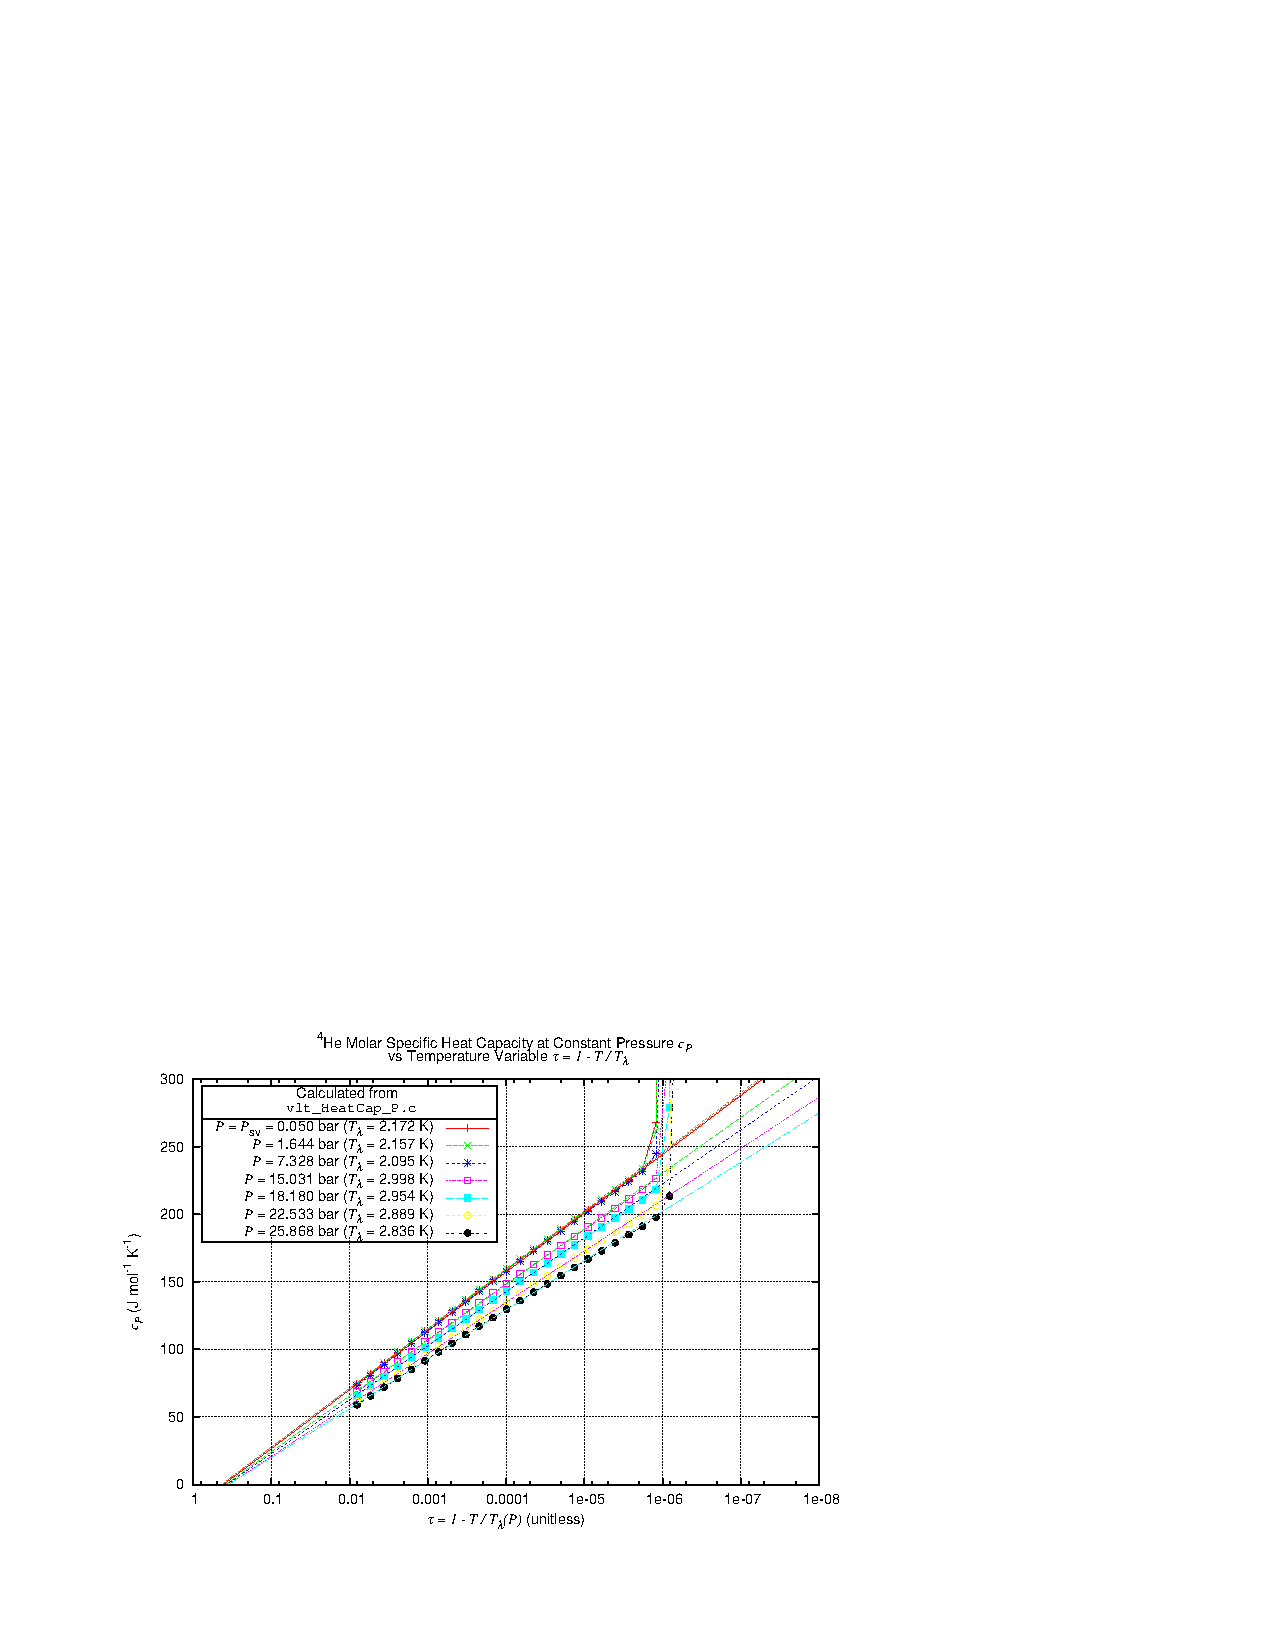
\includegraphics[width=6cm,viewport=54 53 410 300]{plot_vlt_HeatCap_P_DK0_5e-07_CpVsTv_AhlersCompare.pdf}\newline
  \verb|plot_vlt_HeatCap_P_DK0_5e-07_|\newline
  \verb|CpVsTv_AhlersCompare.pdf|
\else
  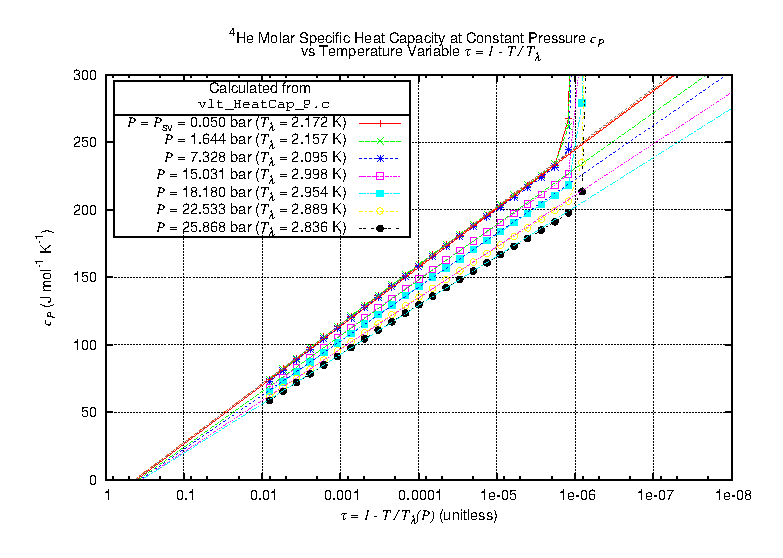
\includegraphics[width=8cm]{plot_vlt_HeatCap_P_DK0_5e-07_CpVsTv_AhlersCompare.ps}\newline
  \verb|plot_vlt_HeatCap_P_DK0_5e-07_|\newline
  \verb|CpVsTv_AhlersCompare.ps|
\fi
&
 \\
\ifpdf
  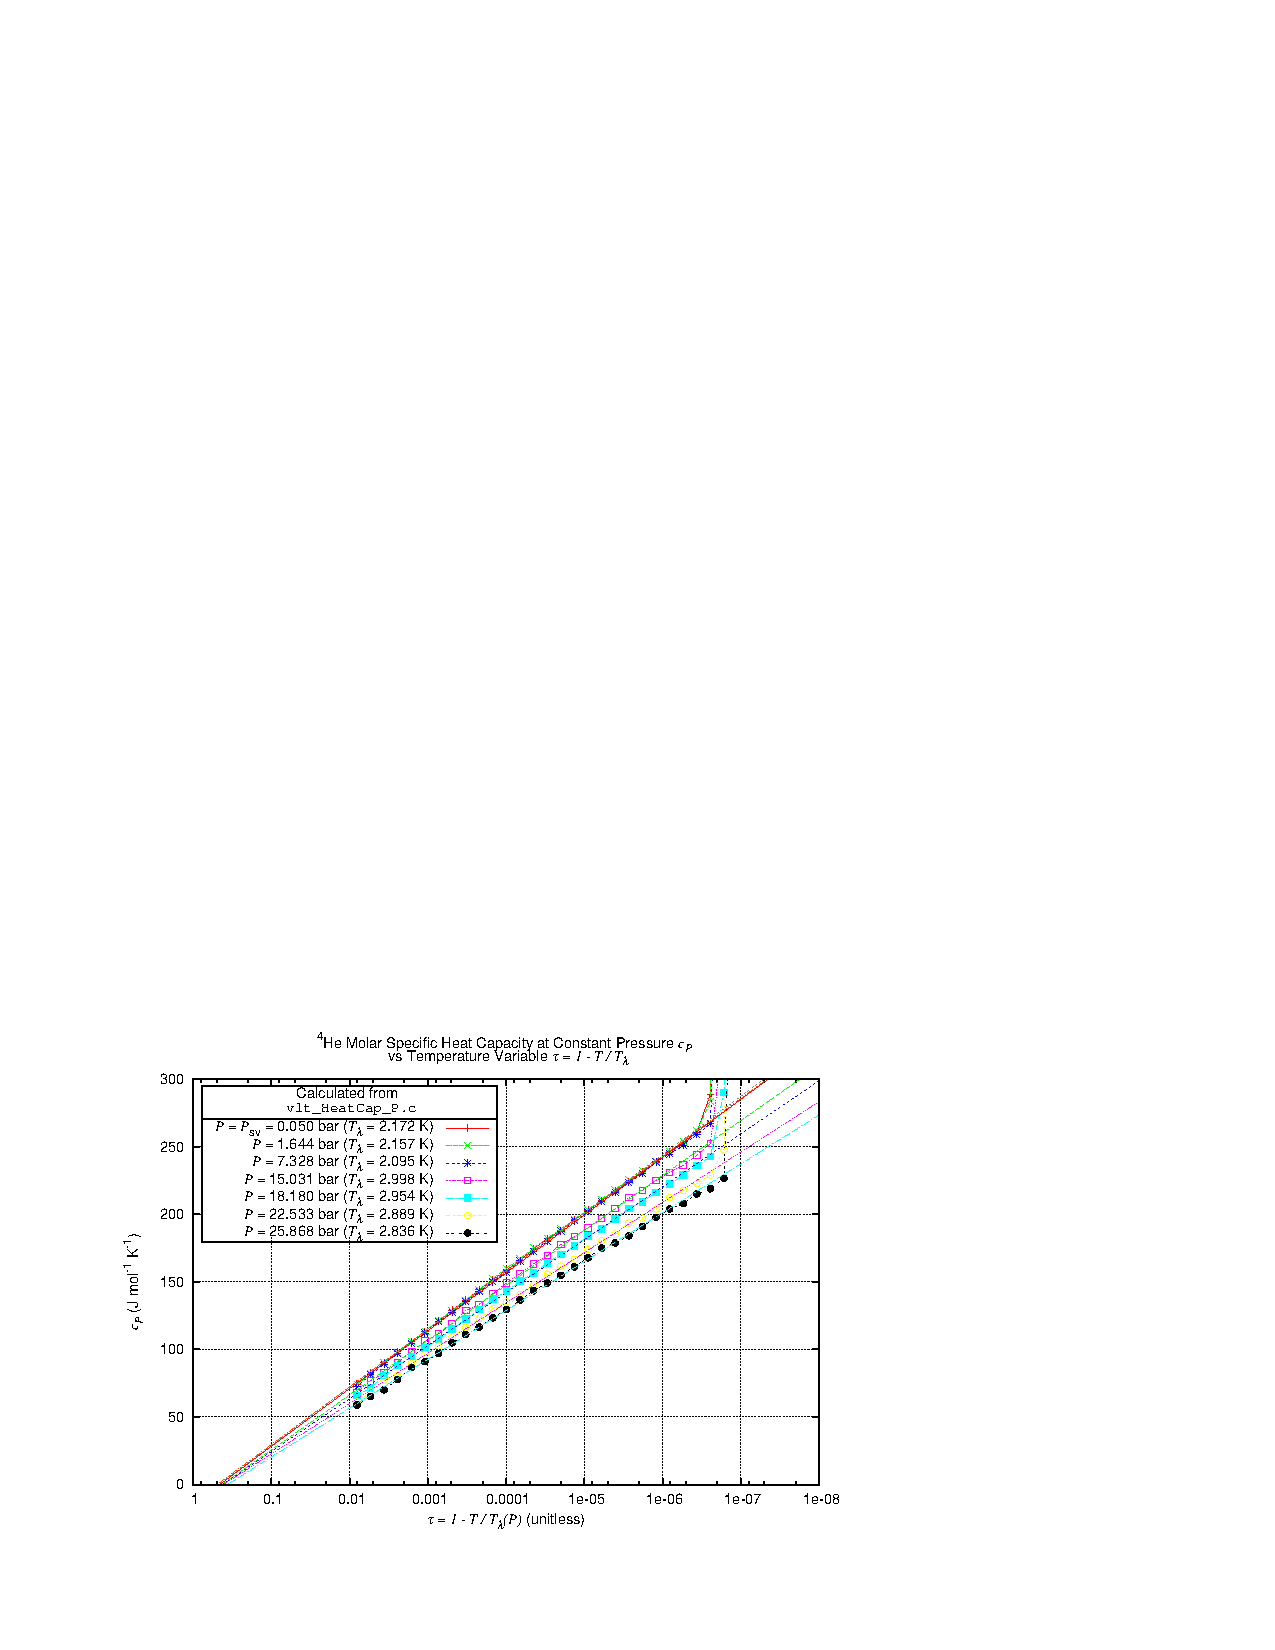
\includegraphics[width=6cm,viewport=54 53 410 300]{plot_vlt_HeatCap_P_DK0_1e-07_CpVsTv_AhlersCompare.pdf}\newline
  \verb|plot_vlt_HeatCap_P_DK0_1e-07_|\newline
  \verb|CpVsTv_AhlersCompare.pdf|
\else
  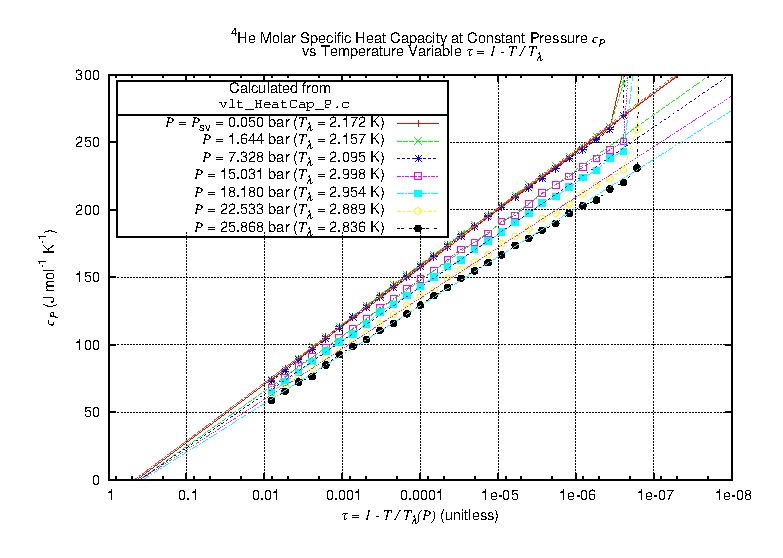
\includegraphics[width=8cm]{plot_vlt_HeatCap_P_DK0_1e-07_CpVsTv_AhlersCompare.ps}\newline
  \verb|plot_vlt_HeatCap_P_DK0_1e-07_|\newline
  \verb|CpVsTv_AhlersCompare.ps|
\fi
&
 \\
\end{tabular}
\end{center}


\end{document}